\chapter{Background}
This chapter will give some background on important algorithms and file formats used in this project. It will also give an introduction to the snow simulator.

\section{Search Algorithms and A* Shortest Path Search Algorithm}
Finding the shortest path between nodes in a graph is an old and heavily researched problem. The problem can be stated like this: Given a weighted graph $G = (V,E)$ with edges $E$ and vertices $V$, and a weighting function $w(e) = w(v_i, v_j)$ of edge $e = (v_i, v_j)$, find the path from $v_a$ to $v_b$, that solves the minimization problem
\begin{equation}
\min_{\mbf P} \left\{ \sum_{e\in \mbf{p}} w(e) \right\}
\end{equation}
over all paths $\mbf P$ between nodes $v_a$ and $v_b$.\cite{shortestpath}

\subsection{Solving shortest path problems}
There are many algorithms to solve the minimization problem of finding the shortest path. There are two main categories: Single-source, and all-pairs. Single-source solves the shortest path algorithm for a single source node $a$, to one or all other nodes. All-pairs finds, as the name suggests, the shortest path between all the nodes in the graph. In this project, we are concerned about the single-source shortest path algorithms. In particular, we are interested in finding the shortest path between one node $v_a$ to another single node $v_b$.

\subsubsection{Dijkstra's algorithm}
One of the most well known and efficient single-source algorithms when we assume that we have no knowledge of the graph, is Dijkstra's algorithm. Dijkstra's algorithm is descriped in algorithm \ref{alg:dijkstra}. The basic idea behind the algorithm is to always choose to look at the neighbors of the node currently closest to the starting node that has not yet been explored. To retrieve the actual path, we keep a pointer to the predecessor of each node, which is updated once a better path to that node has been found. 

\begin{algorithm}
\begin{algorithmic}
\STATE Initially, set the distance to the source $d(v_a)=0$ and for all other nodes $d(v_i) = \infty$.
\STATE Let $\pi(v)$ be the predecessor to node $v$; initially, $\forall v (\pi(v) = \mbox{none})$ 
\STATE Put all nodes $v_i$ in a priority queue, sorted on $d(v_i)$.
\WHILE {$|Q| > 0$}
    \STATE $v := \mbox{next node in Q}$
    \STATE $Q:= Q - \{v\}$
    \FORALL{neighbors $w$ of $v$}
        \IF{$d(v)+w(v,w) < d(w)$}
            \STATE $d(w) :=  d(v)+w(v, w)$.
            \STATE $\pi(w):= v$
        \ENDIF
    \ENDFOR
\ENDWHILE
\end{algorithmic}
\caption{Pseudocode for Dijkstra's algorithm}
\label{alg:dijkstra}
\end{algorithm}

After the algorithm finishes, we have the total cost of the shortest paths from the source $v_a$ to all other nodes. The time complexity, when implemented efficiently with a fibonacci heap, is $O(|E|+|V|\log |V|)$\cite{fibodijkstra}. One useful observation is that the shortest path to the node we pick from the queue is optimal; this is due to the fact that all other nodes in the queue has a larger or equal distance from $v_a$, and thus, assuming non-negative edges, we can not hope to find a better path.. Because of this, if we are only interested in the path from $v_a$ to $v_b$, we can stop the algorithm once we pick $v_b$ from the queue. 

\subsubsection{Utilizing knowledge about graph topology: A*}
In many practical cases, we have specific knowledge about the graph topology. For instance, if we seek to find the shortest path from the city of Oslo to Trondheim, we know, for instance, that if we move in the right direction (i.e. north), we are most probably closer than we were, and we know that we need to travel AT LEAST the straight line distance from Oslo to Trondheim. This kind of knowledge can be utilized in making more efficient single-source, single-destination shortest path algorithms, by computing heuristics on the cost from each node to the goal. One such algorithm is A*.\cite{astar}

A* is an extension of Dijkstra's algorithm. We define $g(x)$ as the distance from the start node $v_a$ to node $x$ ($g(x)$ is the same as $d(x)$ in Dijkstra's algorithm, but it is common to denote this function as $g(x)$ in literature). We also define the heuristic $h(x)$ as an {\textit admissive} (optimistic) and {\textit consistent} (monotone) estimate of the cost from node $x$ to the goal node $v_b$. That the heuristic is optimistic simply means that it never over-estimates the distance left to the goal, i.e. $h(x) \leq h^*(x)$, where $h^*(x)$ is the {\textit optimal} heuristic function, that give the exact cost from node $x$ to the goal node $v_b$. That the heuristic is consistent, means that the search will never take a step back. This is described later.

Combining these values gives the {\textit f-cost} $f(x) = g(x)+h(x)$, which is the actual estimate on the distance from the start node $v_a$ to the goal node $v_b$. The algorithm is outlined in algorithm \ref{alg:astar}.

\begin{algorithm}
\begin{algorithmic}
\STATE Maintain a queue $OPEN$ and a set $CLOSED$. 
\STATE Initially, $OPEN = \{v_a\}$ and $CLOSED = \emptyset$. 
\STATE Let $\pi(v)$ be the predecessor to node $v$; initially, $\forall v (\pi(v) = \mbox{none})$ 
\WHILE {$|Q| > 0 \land v_b \notin CLOSED$}
    \STATE $v := \mbox{node with smallest f-cost in OPEN}$
    \STATE $OPEN:= OPEN - {v}$
    \STATE $CLOSED := CLOSED + \{v\}$
    \FORALL{neighbors $w$ of $v$}
        \IF{$w \notin CLOSED \land w \notin OPEN$}
            \STATE Put $w$ in the $OPEN$ queue.
        \ELSIF{$w \in OPEN \wedge g(v)+w(v,w) < g(w)$}
            \STATE $g(w) := g(v)+w(v,w)$
        \ENDIF
    \ENDFOR
\ENDWHILE
\end{algorithmic}
\caption{Pseudocode for A* shortest path algorithm}
\label{alg:astar}
\end{algorithm}

The main difference from the regular Dijkstra's algorithm, is how nodes are picked from the queue. Instead of picking the node with the lowest $g(x)$ as we do with Dijkstra, we pick the node with the lowest f-cost, $f(x) = g(x) + h(x)$. This way we prefer nodes that are "closer" to the goal. As a side note, if we set $h(x)=0$, the A* algorithm is reduced to Dijkstra's algorithm. If we use the example of finding the shortest route from Oslo to Trondheim, if we use Dijkstra, nodes will be expanded in all directions, i.e. Dijkstra will search both south, west and east, which is unneccesary work. If we instead use A*, nodes south of Oslo may still have a small distance from the start, but will have a higher $h(x)$ than those to the north, and thus may not be selected for expansion. Figure \ref{fig:astar_vs_dijkstra} shows the expanded nodes for a simple shortest path problem where $w(v,w)=1$ for all pairs of neighbors $v,w$, and the neighbors are the neighboring four nodes.

\begin{figure}[ht]
\centering
\subfloat[A* expansions]{\includegraphics[width=0.40\textwidth]{figure/astar_expansion}}
\qquad
\subfloat[Dijkstra expansions]{\includegraphics[width=0.40\textwidth]{figure/dijkstra_expansion}}
\caption{Expanded nodes in A* vs. Dijkstra}
\label{fig:astar_vs_dijkstra}
\end{figure}

\subsubsection{Designing the heuristic. Admissibility and consistency}
In order to guarantee that the A* algorithm is optimal, the heuristic function $h(x)$ must be admissible and consistent\cite{astar}. That $h(x)$ is admissible means that $h(x) \leq h^*(x)$ where $h^*(x)$ is the optimal heuristic that gives the exact distance to the goal from a node $x$. More intuitively, this means that $h(x)$ is an {\textit optimistic} estimate of the cost: the estimate is at most the actual cost. For pathfinding in euclidean space, e.g. in $\mathbb{R^3}$, an admissible heuristic is the straight line distance to the goal; the actual cost to the goal may, however, be higher due to obstacles.

A consistent, also called monotonic heuristic is a heuristic that fulfills the requirement $h(x) \leq w(x,y) + h(y) \Leftrightarrow h(x)-h(y) \leq w(x,y)$. This means that we will never take a step back, because the cost of getting to $y$ from $x$ is greater (or equal to) the difference in the estimates. This implies that if $x$ is the node being explored, we can never find a better $g(x)$ by going through $y$ from $x$; we will always have a monotonically increasing total cost for the best path, as the search goes on. The straight line distance in euclidean space $\mathbb{R^n}$ is a consistent heuristic for the shortest path between two points, because moving in any direction will give a greater or equal total f-cost for the path. It is equal if there is no obstacles, greater if there are, because then we are no longer moving in a straight line.

What heuristic to choose is highly dependent on the problem. For finding the optimal driving route, the euclidean distance to the goal is sufficient. This is also true for the problem of finding a trajectory through a terrain, as is the case in this project. For solving the 8-puzzle, the sum of the manhattan distances of each brick may be an acceptable heuristic. In general, a more accurate heuristic is more expensive to compute, but will also most likely be more efficient in terms of the number of nodes expanded.

\subsection{Applications of shortest path algorithms}
In general, shortest path algorithms solve the minimization problem of finding the path of least cost from a start node $v_a$ to $v_b$. Applications for such algorithms are numerous. Examples are: finding the fastest driving route given a map, finding the best route for a network packet, find the optimal solution to a particular game (e.g. Rubik's cube), and, part of what this project is about, find the best path through a terrain for generating a road trajectory. All that is required, is to express the problem as a weighted graph, and also if using A*, design an admissible and consistent heuristic. 

\section{GPU computing}
Although this project is not particularly about GPU computing, the snow simulator is real-time much because the heavy computation of simulating the wind field and updating the particle velocities and positions are implemented on the GPU. Because of that, the topic of GPU computing is still relevant for this project. This section will describe the capabilities of the GPU, its architecture, and logical layout when used for general purpose computing. We will mainly focus on NVIDIA GPUs here because that is what has been used traditionally in the snow simulator, but the concepts are transferrable to GPUs from other vendors.

\subsection{Physical layout of a GPU}
GPUs (Graphics Processing Units) are accellerators originally intended for highly efficient rendering of 3D graphics on a computer. Rendering is a highly parallel process, where each pixel can be rendered more or less independently from every other pixel. Because of this, GPUs are designed to be highly parallel devices with hundreds of simple vector cores where each vector core typically work on a single pixel. All vector cores may access a global memory with a capacity of hundreds of megabytes up to some gigabytes of memory, but there is also a faster cache available which is shared among groups of size 8 to 32 vector cores, depending on the architecture.

\subsubsection{GPU core organization and properties}
A GPU has hundreds of vector cores called {\textit streaming processor cores} (SPs). These cores are grouped into {\textit streaming multiprocessors} (SMs); each SM has between 8 to 32 SPs depending on the architecture; pre-Fermi architectures had 8, while Fermi-GPUs have 32 SPs. 

\subsubsection{Memory model}
All vector cores may access a global memory, analogous to a regular computer's main memory. However, even though the bandwidth is huge (> 100GB/s for modern NVIDIA Tesla GPUs), the latency is enormous, of hundreds of cycles. This neccessitates a closer and faster memory. On NVIDIA GPUs this memory is called \textit{shared memory}. The difference between shared memory and a traditional cache is that shared memory must be managed manually; i.e. movement of words in and out of shared memory is done explicitly in code.

\subsubsection{Improvements with Fermi}

\subsection{General purpose GPU computing}

\subsection{CUDA}

\section{Newton's method}
\label{sec:newtons_method}
Newton's method is a method for solving equations of the form
$$
f(x) = 0
$$
for some function $f(x)$. It takes as input an initial guess for the value of $x$, $x_0$, and then computes
\begin{equation}
x_{n+1} = x_{n} - \frac{f(x_n)}{f^\prime(x_n)}
\end{equation}
This process is repeated until $|f(x_n)| < \epsilon$, where $\epsilon$ is the tolerance of error. 

The way Newton's method works is that for every iteration, it draws a straight line from the current estimate of $x$, $x_n$, in the direction of the tangent of the curve at $x_n$, and computes the intersection with the line $y=0$. $x_{n+1}$ is then the value of $x$ at that intersection point. Then the process is continued until convergence. 

TODO: FIGURE

Newton's method typically has quadratic convergence\cite{newton}. However, note that Newton's method may not always converge, depending on the choice of the initial guess $x_0$, and the properties of the function. For instance, if a function has a derivative of zero, or if the derivative is otherwise badly behaved near the root, we may fail to find a root using this method. An example is the function $f(x)=\cos(x)$; an initial guess of $0$ gives division by zero, and other guesses causes the next guess to overshoot due to the nature of the function and its derivative.

\section{Clothoids and clothoid splines}
\label{sec:back_clothoid}
Clothoids, or Euler spirals or Cornu spirals as they are also called, is a class of parametric curves that is often used in road modelling and planning due to their pleasant properties with regards to curvature. The curvature changes linearly with respect to the position along the curve, which gives smooth transistions into curves in the road. A clothoid is described by the parametric curve
\begin{equation}
x(t) = aC(t),\  y(t) = aS(t) 
\label{eq:clothoid}
\end{equation}
where $a$ is a scaling factor, and $C(t)$ and $S(t)$ are the Fresnel integrals
\begin{align}
C(t) =& \int_0^t \cos\left(\frac{\pi}{2}s^2\right) ds \label{eq:fresnel_c}\\
S(t) =& \int_0^t \cos\left(\frac{\pi}{2}s^2\right) ds \label{eq:fresnel_s}
\end{align}
and the curvature of a clothoid curve is given by 
\begin{equation}
\kappa(t) = \frac{\pi t}{a},\ \kappa(\theta) = \frac{\sqrt{2\pi\theta}}{a}
\label{eq:clothoid_curvature}
\end{equation}
A plot of a clothoid is shown in figure \ref{fig:back_clothoid}, plotted from $t=0$ and upwards. Note that in many applications of clothoid curves, in particular in road trajectory computation, only the first part of the curve is used, as we will see later on.

\begin{figure}[ht]
\centering
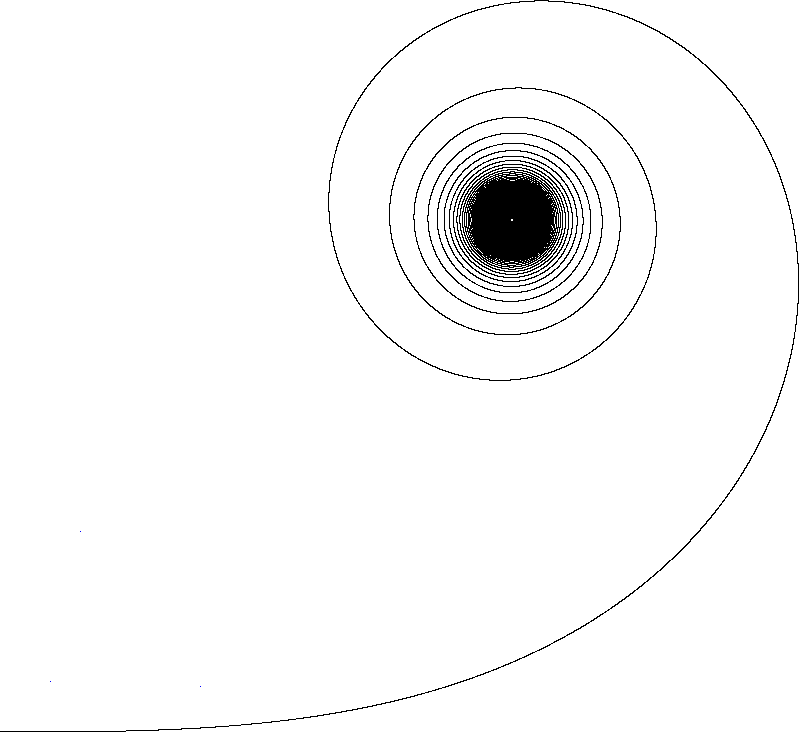
\includegraphics[width=0.4\textwidth]{figure/cornu}
\caption{Plot of a clothoid}
\label{fig:back_clothoid}
\end{figure}

\subsection{The fresnel integrals}
A commonly used form of the Fresnel integrals is given by equations \ref{eq:fresnel_c} and \ref{eq:fresnel_s}, where the parameter is the position along the curve $t$. Alternative forms of these integrals are given by using a point's tangent angle deviation $\theta$ from the beginning of the curve at $t=0$ as a parameter instead of $t$, and is given as\cite{clothoid}\cite{mathhandbook}
\begin{align}
C_2(\theta) =& \frac{1}{\sqrt{2\pi} }\int_0^\theta \frac{\cos(u)}{\sqrt{u}} du\label{eq:fresnel_c2}\\
S_2(\theta) =& \frac{1}{\sqrt{2\pi} }\int_0^\theta \frac{\sin(u)}{\sqrt{u}} du\label{eq:fresnel_s2}
\end{align}
These two forms are equivalent, with\cite{mathhandbook}
\begin{align}
C(t) =& C_2\left(\frac{\pi}{2}t^2\right)\\
S(t) =& S_2\left(\frac{\pi}{2}t^2\right)
\end{align}

The Fresnel integrals can be efficiently computed within an error of less than $\epsilon = 5\cdot 10^{-10}$ without numerical integration, by using polynomial approximations to two functions $f(t)$ and $g(t)$, and then rewriting the integrals as\cite{fresnel}
\begin{align}
C(t) =& \frac{1}{2} + f(t)\sin\left(\frac{\pi}{2}t^2\right) - g(t)\cos\left(\frac{\pi}{2}t^2\right)\\
S(t) =& \frac{1}{2} - f(t)\cos\left(\frac{\pi}{2}t^2\right) - g(t)\sin\left(\frac{\pi}{2}t^2\right)
\end{align}
where
\begin{align}
f(t) = \sum_{n=0}^{11} f_nt^{-2n-1}, g(t) = \sum_{n=0}^{11} g_nt^{-2n-1}
\end{align}
where values for $g_n$ and $f_n$ is given in appendix \ref{app:fresnel}, as well as in \cite{fresnel}. 

\subsection{Notation}
The notation used for this section is based on \cite{clothoid}. The points where clothoid pairs meet with zero curvature will be called \textit{connection points} or \textit{connection vertices}. A clothoid pair is made up by three points; connection points ${\mbf P}_0$ and ${\mbf P}_1$, and control vertex ${\mbf V}$. The vertices are labeled such that $||{\mbf P}_0-{\mbf V}||_2 \geq ||{\mbf P}_1-{\mbf V}||_2$. The vector ${\mbf V} - {\mbf P}_0$ is called ${\mbf g}$ and ${\mbf P}_1-{\mbf V}$ is called ${\mbf h}$; the lengths are referred to as $g$ and $h$, respectively.

The clothoids starting at ${\mbf P}_0$ and ${\mbf P}_1$ are labelled $A_0$ and $A_1$ respectively; any straight line segment that has been appended before $A_0$ is referred to as $S$. The lengths of these curves are $|A_0|$, $|A_1|$ and $|S|$, respectively. The control vertices in a spline with $n$ vertices are referred to as ${\mbf v}_0, ..., {\mbf v}_n$, and the connection points are referred to as ${\mbf p}_0, ..., {\mbf p}_{n-1}$. Note the difference between ${\mbf p}_0$ as the first connection point in the spline, and ${\mbf P}_0$ as the point local to a clothoid pair.

TODO: FIGURE

\subsection{Clothoid splines}
\label{sec:clothoid_spline}
Clothoids can be used to form splines, given a set of control points $\mbf{v}_1, \mbf{v}_2, ..., \mbf{v}_n$.\cite{clothoid} One way of achieving this is first by noting that clothoids have a curvature in the beginning of the curve $\kappa(0) = 0$. Assume that we are given three points $\mbf{V}$, $\mbf{P}_0$ and $\mbf{P}_1$, and the tangent vectors of ${\mbf P}_0$ ${\mbf P}_1$ are ${\mbf T}_0$ and ${\mbf T}_1$, respectively. If we can find a pair of clothoids $A_0$ and $A_1$ that start at $\mbf{P}_0$ and $\mbf{P}_1$, respectively, in the direction of their tangents, so that they are joined at some point $\mbf{P}$ with equal curvature, then we can construct a spline using three or more control points.\cite{clothoid} 

\begin{figure}[ht]
\centering
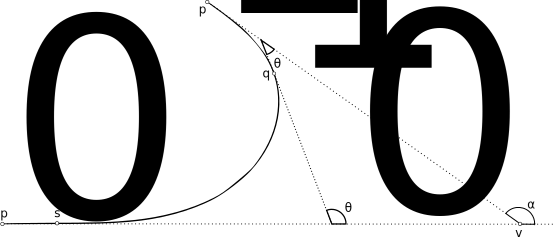
\includegraphics[width=\textwidth]{figure/clothoid_pair}
\caption{Clothoid pair that can be used as a spline segment. $\mbf{q}$ marks where the clothoids are joined, and $\mbf{s}$ marks where a straight line segment is appended.}
\label{fig:clothoid_pair}
\end{figure}


The first step in constructing the spline is to define the vertices where the clothoid pairs meet with zero curvature. One way of choosing these is to use the first and last control vertex as the first and last vertex, and use the midpoint between two control vertices for all the middle points. This is a typical way of doing it, although there may be other ways of choosing the connection vertices. The tangents of each point is chosen so that the last tangent in a clothoid pair points in the direction of the control vertex $\mbf{v}$ from $\mbf{P}_1$, and the very first tangent is chosen in the direction of $\mbf{v}$ from $\mbf{p}_0$. 
%Now, for each control vertex, we may define a clothoid pair from that vertex, and its adjecent connection vertices. 

\subsubsection{Finding clothoid pairs}
Given the three points $\mbf{v}$, $\mbf{P}_0$ and $\mbf{P}_1$ where the tangent vectors of ${\mbf P}_0$ ${\mbf P}_1$ are ${\mbf T}_0$ and ${\mbf T}_1$, respectively, how can a pair of clothoids be found that satisfies the continuity of the curvature at the meeting point, and the initial direction given by the tangent vectors? Label ${\mbf P}_0$ and ${\mbf P}_1$ so that $||{\mbf P}_0-\mbf{v}||_2 > ||{\mbf P}_1-\mbf{v}||_2$, and call the longer edge $g$ and the shorter one $h$. Let $k=g/h$ be the ratio of their lengths. Let $\alpha$ be the angle between these two edges, as shown in figure \ref{fig:clothoid_pair}. Then, if
\begin{equation}
\frac{k + \cos{\alpha}}{\sin \alpha} < \frac{C_2(\alpha)}{S_2(\alpha)}
\label{eq:clothoid_asymmetry_condition}
\end{equation}
then such a pair of clothoids exist.\cite{clothoid} Finding this pair is then done by computing the tangent angle deviation $\theta$ for the meeting point for both clothoids, $\theta_0$ and $\theta_1$, or in other words, find $\theta_0$ and $\theta_1$ such that $\theta_0 + \theta_1 = \alpha$ and $\kappa_{A_0}(\theta_0) = \kappa_{A_1}(\theta_1)$. This is done by solving the equation 
\begin{align}
\sqrt{\theta}[C(\theta)\sin(\alpha) - S(\theta)(k+\cos(\alpha)] + \sqrt{\alpha-\theta}[S(\alpha-\theta)(1+k\cos(\alpha)) - kC(\alpha - \theta)\sin(\alpha)] = 0\label{eq:theta0equation}
\end{align}
for $\theta_0$. For solving this equation, \cite{clothoid} suggests Newton's method or the bisection method. Finding $\theta_1$ is then simply $\theta_1 = \alpha-\theta_0$.

Finally, we must compute the scaling factors for $A_0$ and $A_1$, that is, $a_0$ and $a_1$, respectively. Again referring to \cite{clothoid}, this is done by solving the equation
\begin{align}
a_0C(\theta_0)+a_0\sqrt{\frac{\alpha-\theta_0}{\theta_0}}C(\alpha-\theta_0)\cos(\alpha) + a_0\sqrt{\frac{\alpha-\theta_0}{\theta_0}}S(\alpha-\theta_0)\sin(\alpha) = g+h\cos(\alpha)\label{eq:a0equation}
\end{align}
for $a_0$. This is a simple rearrangement of terms since $\theta_0$ and all other values are known at this point. To find $a_1$, we use the formula\cite{clothoid}
\begin{equation}
a_1 = a_0 \sqrt{\frac{\theta_1}{\theta_0}} = a_0 \sqrt{\frac{\alpha - \theta_0}{\theta_0}}
\label{eq:a1equation}
\end{equation}

Now we have all we need to define the clothoid pair given by the three points: The scaling factors $a_0$ and $a_1$, and the tangent angle deviation of the curves at their endpoints $\theta_0$ and $\theta_1$.

\subsubsection{Appending straight line segments}
There may be a significant asymmetry between the lengths of $g$ and $h$; i.e., given a control vertex $\mbf{v}$ and two points $\mbf{p}_0$ and $\mbf{p}_1$, $||{\mbf P}_0-\mbf{v}||_2$ and $||{\mbf P}_1-\mbf{v}||_2$ may be very different. It is easy to see that if this is the case, the inequality \ref{eq:clothoid_asymmetry_condition} may no longer hold and we may not be able to find a clothoid pair for these three points. Because the curvature at the joints between clothoid pairs are zero, the same as a straight line, this can be solved by simply appending a straight line, and "moving" the starting point furthest away from ${\mbf v}$ closer, so that the asymmetry is reduced. Moving it so that $g=h$ results in a symmetric pair of clothoids, i.e. one clothoid is simply a reflection of the other.\cite{clothoid}

To achieve this, assume that the point furthest away from ${\mbf v}$, i.e. the point defining $g$, is labelled ${\mbf P}_0$. Then we may define a symmetry parameter $\tau\in [0, 1)$ that determines how close to ${\mbf v}$ we wish to move ${\mbf P}_0$. $\tau=0$ gives perfect symmetry, while any other value of $\tau$ gives different degrees of asymmetry, up to the limit determined by \ref{eq:clothoid_asymmetry_condition}. The limit of the size of $g$ is given by rearranging the inequality \ref{eq:clothoid_asymmetry_condition}, and changing the inequality sign with an equality sign:
\begin{equation}
g_{lim} = h\left(\frac{C(\alpha)}{S(\alpha)}\sin(\alpha) - \cos(\alpha)\right)
\end{equation}
Then, ${\mbf P}_0$ is moved to 
\begin{equation}
{\mbf P}_0^\prime = {\mbf v}-((1-\tau)h + \tau g_{lim}){\mbf T}_0
\end{equation}
and the region of the curve between ${\mbf P}_0$ and ${\mbf P}_0^\prime$ is now described by a straight line between these two points. 


\section{Road generation}
Roads can be generated in a number of ways; city street networks can be generated using using Lindenmayer systems\cite{citymodelling}, and shortest path algoriths like A* can be used to generate roads through a terrain, and this method may even be extended to generating hierarchical roads.\cite{roadgen}\cite{roadgen2}
Generating realistic roads is more often than not non-trivial due to the many variables that determine if a road is "good" or not. For instance, different types of roads (e.g. highways, country roads) may have different tolerance to changes in elevation and curvature, and the tradeoffs of going up a steep slope or making a longer, more curvy road around that slope must be weighted. In this section we will first look at how we can formulate the problem of generating a road through a terrain as a shortest-path problem as described by \cite{roadgen}, and lastly we will discuss the details about the trajectory computation and road modelling given a discrete shortest path.
%A cost function controls the road trajectory we get

\subsection{Formulating road generation as a shortest-path problem}
\label{sec:roadgen_shortestpath}
Road generation can be formulated as a shortest-path problem in the following manner. First, discretize the terrain into a grid of elevation points. Each of these points is then a node in the graph. Conveniently enough, these points are also in $\mathbb{R}^3$ $(x,y,height)$, which makes designing heuristics for A* easier.

Next, we must define the edges of the graph. Those edges define, naturally, which nodes that can be reached from each node. The most naive ways of defining this neighborhood is either to choose ALL nodes to be reachable from every other node, or only the immediate eight neighbors. The first approach would be computationally infeasible due to the sheer amount of nodes in the graph. The other approach has a severe restriction on angles (the so-called limit on direction problem\cite{roadgen}), as the pathfinding algorithm can only take turns in multiples of 45 degrees, resulting in a fairly jagged path. 

The solution to this problem of limit on direction, as presented in\cite{roadgen}, is to not only use the immediate neighbors, but use a neighborhood mask to define the neighbors. This mask is defined as follows: The neighbors of a point $p_{a,b}$ is defined as all points $p_{a+i,b+j}$ where $i,j$ are integers, $gcd(i,j) = 1$ and $i,j \in [-k,k]$. That $gcd(i,j)=1$ requirement is not a requirement for correctness, but to avoid unneccesary cost function evaluations for overlapping paths. Figure \ref{fig:neighbormask} illustrates the neighborhood of a grid point with a mask size of $k=2$.

\begin{figure}[ht]
\centering
\includegraphics[width=0.5\textwidth]{figure/neighbormask}
\caption{Neighborhood of grid point (middle).}
\label{fig:neighbormask}
\end{figure}

In order to define the weights of each edge, we define the cost of building an infinitesimal portion of road from point ${\mbf p}$, in the direction $\dot{\mbf p}$ and rate of change of the direction $\ddot{\mbf p}$ as $c({\mbf p}, \dot{{\mbf p}}, \ddot{{\mbf p}})$. Now, in order to evaluate the cost of a particular trajectory, simply integrate over the curve as shown in equation \ref{eq:roadcost}. Here, $t_1$ and $t_2$ define the segment end points of the parametric curve defined by the whole trajectory, as illustrated in figure \ref{fig:trajectory_segment}. $t_1$ and $t_2$ correspond to the grid points ${\mbf p}_{i_1,j_1}$ and ${\mbf p}_{i_2,j_2}$, respectively.

\begin{equation}
cost({\mbf p}_{i_1,j_1}, {\mbf p}_{i_2,j_2}) = \int_{t_1}^{t_2} c({\mbf p}(t), \dot{{\mbf p}}(t), \ddot{{\mbf p}})(t) dt
\label{eq:roadcost}
\end{equation}

Evaluating this integral can be done numerically by discretizing the curve into intervals of length $\Delta t$ and using some numerical integration method like the midpoint rule or Simpson's rule.

\begin{figure}[ht]
\centering
\includegraphics[width=0.5\textwidth]{figure/trajectory_segment}
\caption{Trajectory segment}
\label{fig:trajectory_segment}
\end{figure}

\subsection{Cost functions}
There are many potential contributing factors to the cost of a trajectory. One of them is of course road length, where the cost typically increases linearly with the length. In order to get realistic roads, however, using only road length as a cost function is not sufficient, because that would simply generate a nearly straight line from start to goal, which is suboptimal in e.g. a mountainous terrain. Adding an extra cost for slopes, or change in elevation, will cause the road to have curves around steep mountain sides, and roads will generally avoid bumpy terrain. However, this may result in sharp turns because curvature is not taken into account when attempting to avoid elevation changes. This may be alleviated by also taking curvature into account.

Let each of the cost functions, for road length, elevation changes and curvature, and possibly more, be numbered $1, ..., n$ where $n$ is the number of cost functions. Also, let $\mu_i$ be a {\textit transfer function} that maps the measured values of slope, curvature and so on, to the actual cost value. It may be helpful to think of $\mu_i$ as a weighting function, although it may also be unlinear. Then, the cost function can be defined as
$$
C({\mbf p}, \dot{{\mbf p}}, \ddot{\mbf{p}}) = \sum_{i=1}^{n} \mu_i(c_i({\mbf p}, \dot{{\mbf p}}, \ddot{\mbf{p}}))
$$

\subsection{Trajectory computation}
A piecewise linear curve, like the one given by the discrete shortest path A* algorithm described above, is not a good description of the road trajectory, as this gives very sharp turns. Instead, the road trajectory can be modelled as a clothoid spline\cite{roadgen}, which is described in section \ref{sec:back_clothoid}. This gives a pleasant curvature which varies linearly with the position along the curve\cite{clothoid}. Given the discrete shortest path represented by the points ${\mbf p}_0, {\mbf p}_1, ..., {\mbf p}_n$, a clothoid spline can be constructed using these points as control points. The spline starts and ends at the end points (${\mbf p}_0$ and ${\mbf p}_n$). 

\section{The Snow Simulator}
A major part of this project is to extending the snow simulator developed at the HPC lab at NTNU, to support loading meshes (mainly roads, but may be arbitrary meshes). In order to fully integrate the contributions from this project into the snow simulator, it is important to have some background on the way the snow simulator works. Figure \ref{fig:back_snowsim_screenshots} shows the snow simulator in action. This section will first describe the terrain format. Then, wind simulation and particle updates are described briefly.

\begin{figure}[ht]
\subfloat{
    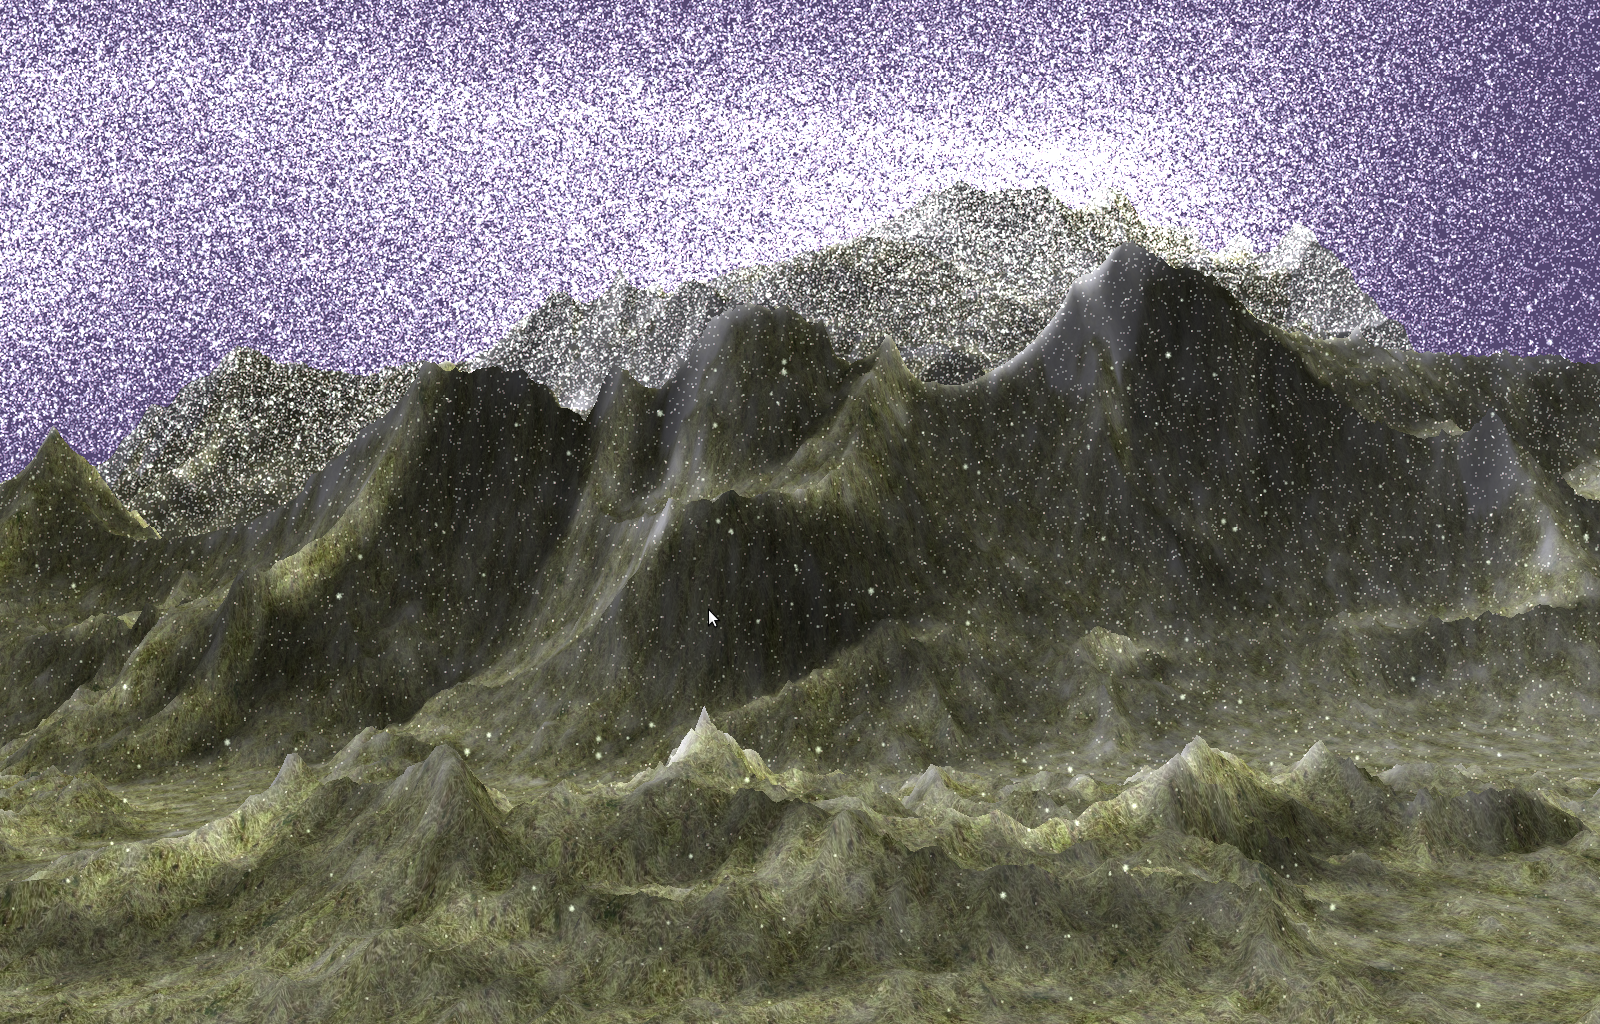
\includegraphics[width=0.5\textwidth]{figure/screenshots/snowsim_plain_start}
}
\subfloat{
    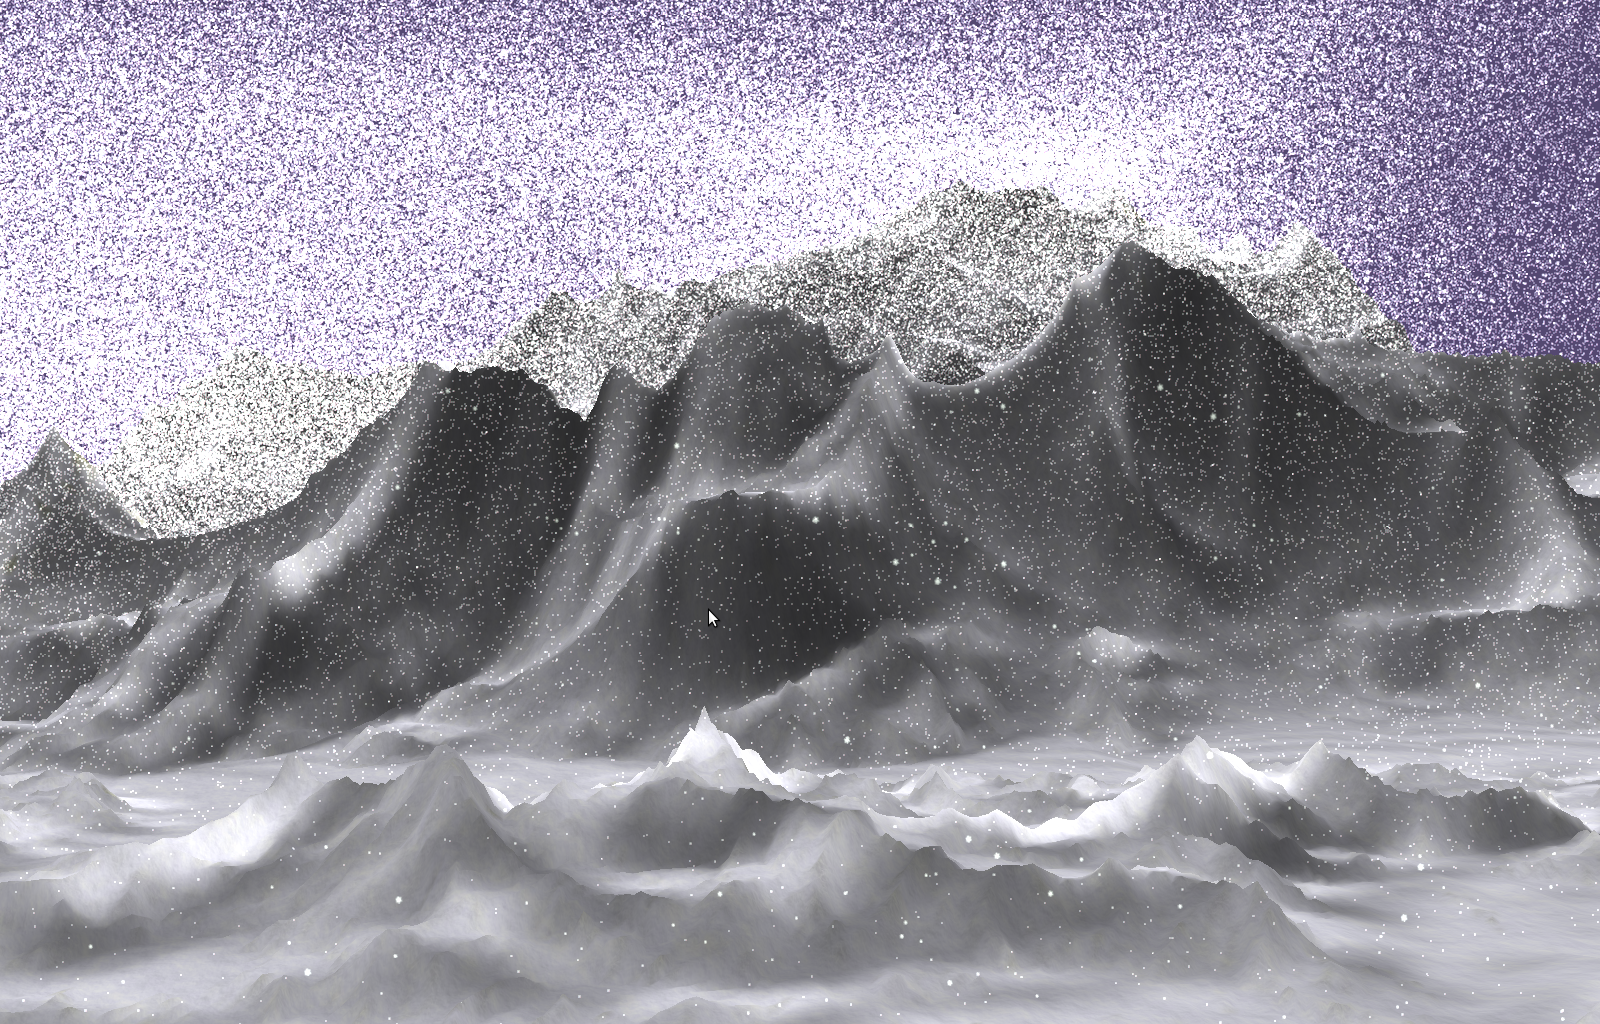
\includegraphics[width=0.5\textwidth]{figure/screenshots/snowsim_plain_end}
}
\caption{A scene before and after being covered with snow}
\label{fig:back_snowsim_screenshots}
\end{figure}

%Also, a few other improvements, discussed in section \ref{sec:impl_snowsim}, have been done. 

\subsection{Terrain}
Terrains are in many applications represented by a height map, which is nothing more than a bitmap of a certain width and height, where each element represent a height in the terrain. In the snow simulator, a 16 bit integer height map is used; this means, each height value is an integer of 16 bits, which is then mapped to an actual height value in the model. 

The height map is stored as raw data, with no header, in row-major order; that is, the elements within a row is stored sequentially in the file, so row 1 is stored first, followed by row 2, etc. The map is loaded by first reading all the values of the file, then generating vertices for a triangle mesh that will be used as rendering. In the original snow simulator that this project aims to extend, the integers are mapped to a floating point value between 0 and 64. This means that a value of zero represents an y vertex position of zero, and a value of $2^{16}-1$ is mapped to a vertex y-position of 64. Figure \ref{fig:heightmap} shows a visualizeation of a height map.

\begin{figure}[ht]
\centering
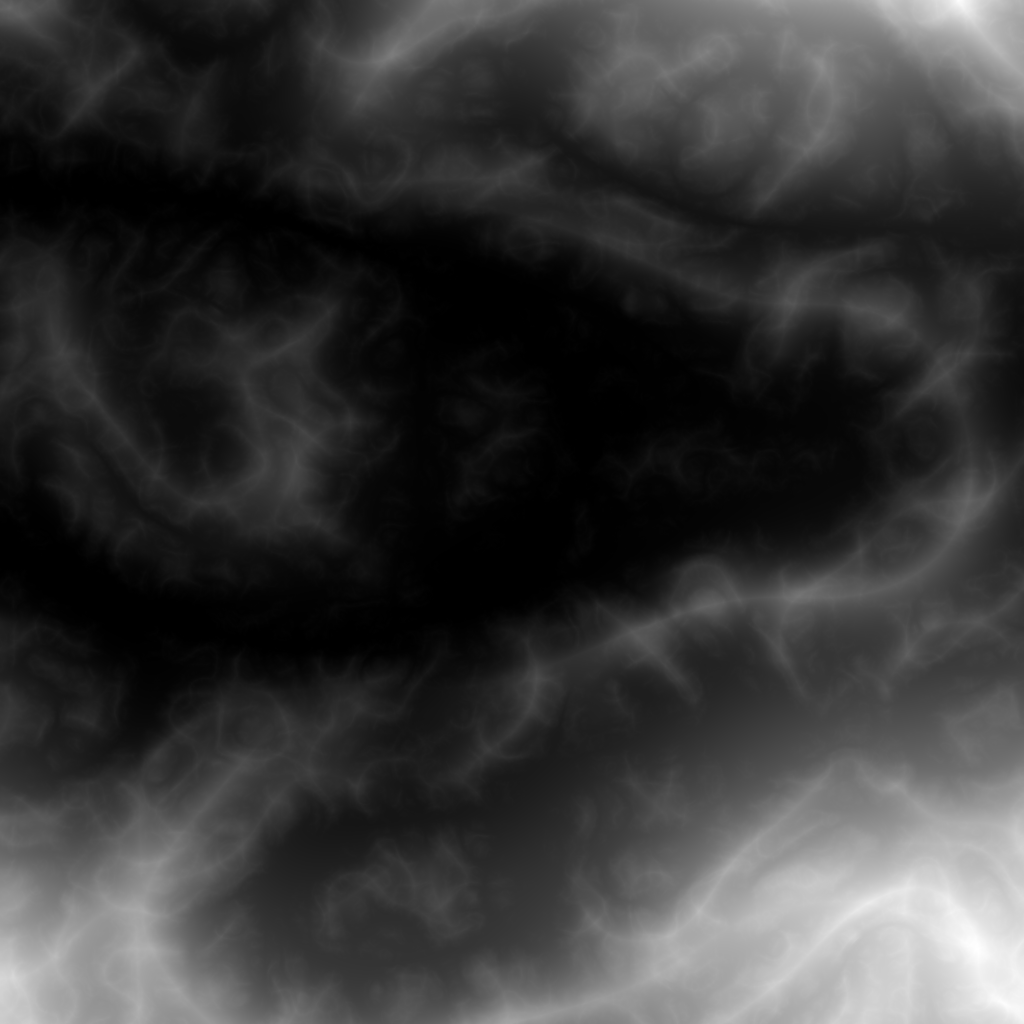
\includegraphics[width=0.5\textwidth]{figure/heightmap}
\caption{A heightmap of a terrain}
\label{fig:heightmap}
\end{figure}

\subsection{Wind simulation}
Wind in the snow simulator is modelled by the incompressible Euler equations, which is derived from the Navier-Stokes equations by setting the viscosity to zero and density to one,
\begin{align}
\nabla \cdot {\mbf u} = & 0\\
\frac{\delta{\mbf u}}{\delta t} = & -({\mbf u}\cdot \nabla){\mbf u} - \nabla{\mbf p}
\end{align}
where ${\mbf p}$ is the pressure, and ${\mbf u}$ is the velocity vector field.

This equation is simulated numerically by first solving for advection (movemenet of the fluid along its own motion), then solving for pressure which involves solving the poisson equation $\nabla^2 p = \nabla\cdot {\mbf u}^*$ (where ${\mbf u}^*$ is a temporary velocity field generated from the advection step), and finally projecting these velocities into a divergence-free (mass conserving) field\cite{snowsim1}.

\subsection{Particle updates}
Snow particles are updated according to their current velocity, wind velocity at their position and gravity.\cite{snowsim1} First, the wind velocity is interpolated from the wind field. Then, a circular velocity of the snow particle is computed, which causes them to rotate around a central axis. Then the accelleration is computed from the drag (a function of the difference between the velocities of the wind and snow particles), and gravity. 

TODO 

\section{USGS DEM Format}
USGS DEM is a file format for storing elevation data. It is a format in human readable ASCII characters, and the files are segmented into blocks of 1024 bytes. There are three types of records in a DEM file: one A-record, which is the header; multiple B-records, where each B-record store one column of elevation data and one C-record, which stores statistics of errors and accuracy of the data.\cite{usgsdem}

The data in a DEM is defined for a quadrangle; i.e. an arbitrary polygon of four vertices. The quadrangle may or may not be an axis-aligned rectangle, but most likely it will be {\textit close} to a rectangle. Oftentimes, the quadrangle attempts to follow the curvature of the earth mapped onto a plane, which gives slightly rotated and skewed rectangles.

Next, I will give an overview of the A and B records of a DEM. The C-record is not relevant for this project.

\subsection{A-record overview}
The A-record is the header of the DEM file, containing data such as the vertices of the quadrangle in world coordinates, total number of columns of data, minimum and maximum elevation in the DEM, units used for the quantities in the file (feet, meters, arc seconds), and so on. It also stores information about resolution in all three dimensions. 

\subsection{B-record overview}
\label{sec:back_brecord}
Each B-record stores one column of data for the height map along with a header for this data. However, since the quadrangle stored in a DEM file may not be quadratic, each column may have different number of elements. The position of the bottom-most point is specified in the header in world coordinates, along with the number of points. One B-block may span more than one 1024-byte block.

Each elevation data point in the B-record is stored as an integer, and may be converted to an actual height value $h_i$ (in meters) by using the following formula for datapoint $y_i$:
$$
h_i = ((e_{max}-e_{min})\cdot y_i+ d_y)\cdot res_y \cdot unit
$$

where $d_y$ is the height datum and $e_{max}$ and $e_{min}$ is the maximum and minimum elevation, respectively. $unit$ is the number of meters per unit specified in the A-record; $unit=1$ for meters, or $0.3048$ for feet.

Details about the layout of the USGS DEM file format can be found in appendix \ref{app:usgsdem}.

\section{RoadXML}
The RoadXML format is an XML based file format used to describe road networks. In addition to describing the trajectories, it also describes the profile of the road (i.e. width, markings, number of lanes, ...) and textures used for rendering.\cite{roadxml} RoadXML is an open format, developed in collaboration with the driving simulation industry and universities. Although RoadXML is a very powerful and extensive format used to describe complex systems with intersections, traffic information, grip, and much more, it is in this project only used as a road trajectory descriptor suitable for generating the road model.


